\documentclass[conference,compsoc]{IEEEtran}
% IEEE S&P 2027, compsoc conference format. US letter; 13pp body + 5pp refs;
% double-blind. Do not alter margins/fonts/spacing (desk-reject triggers).
\usepackage[T1]{fontenc}
\usepackage{amsmath,amssymb,amsthm}
\usepackage{booktabs}
\usepackage{xcolor}
\usepackage{tikz}
\usetikzlibrary{arrows.meta,positioning,fit,backgrounds,calc}
\usepackage[hidelinks]{hyperref}
\usepackage{url}
\setlength{\emergencystretch}{3em} % absorb tight lines in the narrow columns

% IEEEtran does not predefine theorem-like environments; define them.
\newtheorem{proposition}{Proposition}
\newtheorem{lemma}{Lemma}
\newtheorem{assumption}{Assumption}

\newcommand{\ext}{\texttt{a2a.privacy/v1}}

\begin{document}

\title{Privacy Typing for Multi-Tenant Agent Interaction:\\
A Federated, Center-Blind Auditor and an A2A Extension}

\author{\IEEEauthorblockN{Anonymous Author(s)}
\IEEEauthorblockA{Submitted for double-blind review}}

\maketitle

\begin{abstract}
Autonomous agents increasingly delegate work to one another across organizational
boundaries, and protocols such as A2A now standardize how they do so. These protocols carry
no notion of whom a datum concerns or who may receive it, so the resulting
leakage is hard to see: it happens on internal agent-to-agent channels and is
often compositional, emerging from messages that are each individually benign.
Centralized observability offers no remedy, because it must read the very content
that sensitive, cross-organizational deployments will not expose.

We present a federated auditor that detects these leaks from desensitized metadata
it can never invert to content, together with a privacy-typing extension to A2A
that makes the leaks expressible in the first place. By separating the data
subject, the owning principal, and the agent principal, the auditor flags
cross-tenant disclosure, purpose violations, over-forwarding, and cross-tenant
inference, all without reading a message. We prove the center-blind guarantee (the
center learns $O(\log)$ bits per message) and characterize when inference becomes
detectable, then test the system where it is easiest to fool ourselves: on a
benchmark authored by a separate model it keeps perfect precision, and against a
real LLM recipient we confirm that two benign fragments already expose a withheld
attribute, a threat that grows with model capability. On its single-tenant
projection, which is the deployable product, the auditor catches every
internal-channel leak in AgentLeak's 600 scenarios at 0.97 precision with zero
content egress.
\end{abstract}

\begin{IEEEkeywords}
multi-tenant agents, agent-to-agent protocols, privacy auditing, information-flow
control, compositional inference, differential privacy
\end{IEEEkeywords}

\section{Introduction}
Agents are starting to talk to \emph{each other}. Protocols such as A2A (v1.0,
Linux Foundation), MCP, and ACP let agents built by different teams discover
capabilities and delegate work across organizational boundaries. As this fabric
forms, a question with no answer today becomes urgent: \emph{when my agent hands
data to your agent, what did it just share, and was it allowed to?}

This is already a live privacy problem, not a hypothetical one. Production agents
in regulated settings---healthcare schedulers, financial assistants, HR
copilots---increasingly delegate to third-party agents, and a single over-shared
identifier (an SSN, a diagnosis, an account number) crossing that organizational
boundary is a concrete privacy harm under regimes such as HIPAA and GDPR. Our aim
is a deployable safeguard for exactly these real cross-organizational agent
interactions: the system we build runs today, sees no raw content, and---as our
in-the-wild study shows (\S\ref{sec:eval})---catches current agents over-sharing
regulated identifiers in 46--82\% of realistic hand-offs across four open-weight and
frontier models.

Three things make this hard at once. The leakage is where it is least watched:
inter-agent messages leak far more than final outputs, yet no current framework
monitors the internal channel~\cite{agentleak}. It is also compositional, arising
from messages that are each individually benign even when every agent obeys its
own policy~\cite{sumleaks}. And across organizations the parties do not trust one
another: the other agent is the adversary, and no one will route raw content
through a central observer, which is precisely what centralized observability
(LangSmith, Langfuse) requires.

The protocols do not help. We verified against the A2A v1.0 specification that its
data model (\texttt{AgentCard}, \texttt{Task}, \texttt{Message}, \texttt{Part})
has \textbf{no data-governance semantics}: no field marks whom a datum is about,
who owns it, what it may be used for, or which agent may receive it. A2A provides
free-form \texttt{metadata}, an \texttt{extensions} array, and a loosely-specified
\texttt{tenant} field that routes but does not govern.

We close this gap. Our contributions:
\begin{enumerate}
\item \textbf{\ext{}}, a privacy-typing extension carried in \texttt{Part.metadata}
that types every shared datum (owner, subject, sensitivity, category, purpose,
recipient set, hop limit, provenance id) and composes with unmodified A2A.
\item \textbf{A multi-tenant threat model and a center-blind auditor.} We separate
the data subject, owning principal, and agent principal, and detect cross-tenant
disclosure, purpose, hop/TTL, and \emph{cross-tenant inference} from desensitized
metadata the center cannot invert---the privacy-preserving counterpart to
centralized observability.
\item \textbf{A2A-MT}, the first multi-tenant agent-privacy benchmark
(parameterized families, realistic LLM-generated content), plus validation of the
underlying engine on the external AgentLeak benchmark.
\end{enumerate}
Setting every principal equal collapses the system to the \textbf{in-container}
case---one organization auditing its own multi-agent app---so the research result
and a practical product share one implementation (Figure~\ref{fig:arch}).

\begin{figure*}[t]\centering
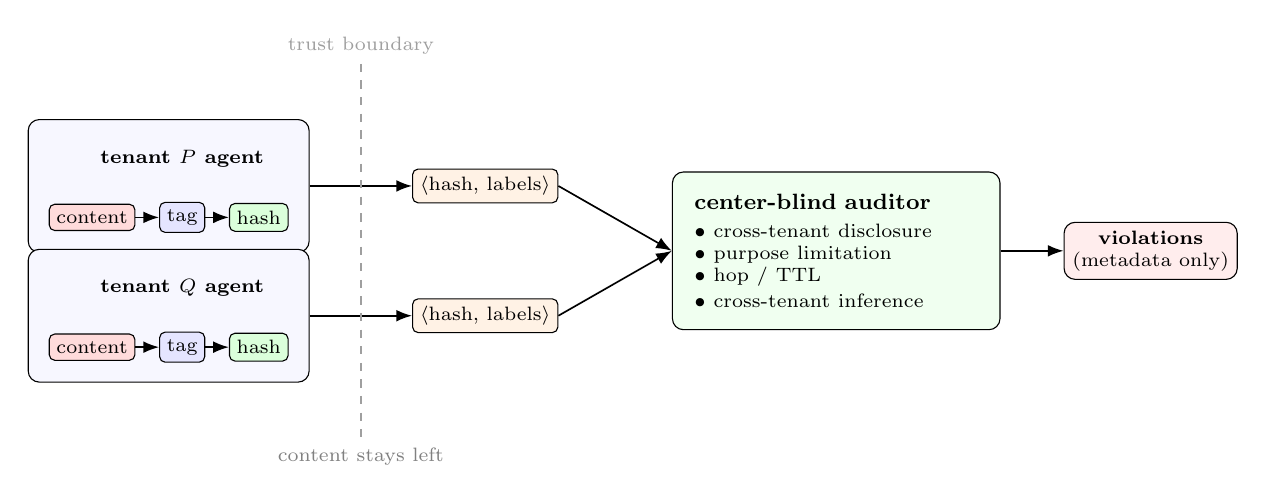
\begin{tikzpicture}[font=\footnotesize,>=Latex,
  pill/.style={draw,rounded corners=2pt,inner sep=2.6pt,font=\scriptsize},
  card/.style={draw,rounded corners,fill=blue!3,inner sep=2.6mm},
  crumb/.style={draw,rounded corners=2pt,fill=orange!10,inner sep=2.6pt,font=\scriptsize},
  ar/.style={-{Latex},semithick}]
% --- in-agent pipelines (content -> tag -> hash) for tenants P and Q ---
\node[pill,fill=red!14] (pc) {content};
\node[pill,fill=blue!10,right=3mm of pc] (pt) {tag};
\node[pill,fill=green!14,right=3mm of pt] (ph) {hash};
\node[above=3.2mm of pt,anchor=south,font=\scriptsize] (ptl) {\textbf{tenant $P$ agent}};
\node[pill,fill=red!14,below=13mm of pc] (qc) {content};
\node[pill,fill=blue!10,right=3mm of qc] (qt) {tag};
\node[pill,fill=green!14,right=3mm of qt] (qh) {hash};
\node[above=3.2mm of qt,anchor=south,font=\scriptsize] (qtl) {\textbf{tenant $Q$ agent}};
\begin{scope}[on background layer]
\node[card,fit=(pc)(ph)(ptl)] (P) {};
\node[card,fit=(qc)(qh)(qtl)] (Q) {};
\end{scope}
\draw[ar] (pc)--(pt); \draw[ar] (pt)--(ph);
\draw[ar] (qc)--(qt); \draw[ar] (qt)--(qh);
\node[draw,rounded corners,fill=green!6,inner sep=2.8mm,text width=36mm,
  right=46mm of $(P.east)!0.5!(Q.east)$,anchor=west] (C)
  {\textbf{center-blind auditor}\\[2pt]
   \scriptsize $\bullet$~cross-tenant disclosure\\
   \scriptsize $\bullet$~purpose limitation\\
   \scriptsize $\bullet$~hop / TTL\\
   \scriptsize $\bullet$~cross-tenant inference};
\node[draw,rounded corners,fill=red!7,inner sep=3pt,align=center,font=\scriptsize,
  right=8mm of C] (V) {\textbf{violations}\\(metadata only)};
\node[crumb,right=13mm of P.east,anchor=west] (eP) {$\langle$hash, labels$\rangle$};
\node[crumb,right=13mm of Q.east,anchor=west] (eQ) {$\langle$hash, labels$\rangle$};
\draw[ar] (P.east)--(eP); \draw[ar] (eP.east)--(C.west);
\draw[ar] (Q.east)--(eQ); \draw[ar] (eQ.east)--(C.west);
\draw[ar] (C.east)--(V.west);
\coordinate (bx) at ($(P.east)+(6.5mm,0)$);
\draw[dashed,gray!75,thick] ([yshift=7mm]P.north-|bx) -- ([yshift=-7mm]Q.south-|bx);
\node[gray!75,font=\scriptsize,anchor=south] at ([yshift=7mm]P.north-|bx) {trust boundary};
\node[gray,font=\scriptsize,anchor=north] at ([yshift=-7mm]Q.south-|bx) {content stays left};
\end{tikzpicture}
\caption{Federated, center-blind architecture. Inside each agent the raw
\textcolor{red!60!black}{content} is \textcolor{blue!60!black}{tagged} and
\textcolor{green!45!black}{hashed} locally; only desensitized edges
($\langle$one-way hash, \ext{} labels$\rangle$)---never content---cross the trust
boundary. The center runs four detectors over this metadata graph and cannot invert
it to content (Lemma~\ref{lem:blind}).}
\label{fig:arch}
\end{figure*}

\section{Background and the governance gap}
An A2A interaction is a sequence of \texttt{Message}s between agents; each carries
\texttt{Part}s (text/data/file) and free-form \texttt{metadata}. The model has no
field for ownership, sensitivity, purpose, or recipient restriction; privacy is
delegated to ``external access control'' that, across tenants, does not exist. We
add the missing layer inside A2A's extension mechanism so it composes with
deployed agents, and audit it with a \emph{federated} architecture: each agent
desensitizes locally; a central auditor reasons over a graph of metadata it can
never invert to content.

\section{Threat model}\label{sec:threat}
\paragraph{Principals.} A single identifier must not conflate three roles: the
\textbf{data subject} (whom a Part is about), the \textbf{owning principal} (who
controls the datum and the originating agent), and the \textbf{agent principal} (an
agent's AgentCard identity). Governance is defined over principals, not agents: a
datum owned by $P$ may reach an agent of $Q$ only if $Q$ is an allowed recipient for
$P$'s stated purpose.

\paragraph{Adversary.} We consider a receiving or forwarding agent of a different
tenant with three capabilities: (A1) it reads every Part routed to it and may
\emph{infer} beyond what is stated; (A2) it may \emph{paraphrase, split, or re-route}
what it forwards; and (A3) a \emph{dishonest sender} may mislabel its own Parts
(suppress tags or forge a subject id), since labels are produced locally. The
adversary controls neither the A2A transport nor other tenants' processes.

\paragraph{Trust assumptions (software baseline).} (T1) \emph{center-blind}: the
auditor detects from desensitized metadata and never sees raw \texttt{Part} content,
and no tenant reveals content to it or to peers; (T2) \emph{honest-but-curious peers}
for the disclosure, purpose, and TTL detectors---agents route truthfully but try to
learn more than authorized; (T3) \emph{A2A transport is given}---we annotate and
audit, not replace. Under T1--T3 the design defeats A1 and A2 (wording and routing
attacks) by construction, because the detectors key on labels and principals, not on
text (\S\ref{sec:eval}); A3 is the residual the baseline does not close.

\paragraph{Closing A3 with forced-embed attestation.} We remove the honest-labeler
assumption with a downloaded, build-pinned component. The labeler and auditor ship as
a fixed build $B$ whose signing key $k_B$ is confined to $B$; a report is
$R=(\mathcal{E},\sigma)$ with $\sigma=\mathrm{Sign}_{k_B}(H(\mathcal{E}))$ over the
center-view edge set $\mathcal{E}$, and the center accepts $R$ only if it verifies
under $B$'s published fingerprint.

\begin{proposition}[Attestation soundness]\label{prop:attest}
If the signature scheme is \textup{EUF-CMA}-secure and $k_B$ is confined to $B$, then
every report the center accepts equals $B$'s output on the sender's actual inputs,
except with negligible probability. Hence a modified labeler that suppresses a tag or
forges a subject id yields a report signed by an untrusted build (wrong fingerprint)
and is rejected, and content tampering changes $H(\mathcal{E})$ and fails
verification. The residual adversary is confined to (i) exfiltrating $k_B$ from
$B$---the case a hardware root of trust (TEE) closes---and (ii) \emph{sub-threshold}
leakage: disclosing strictly less than the detection threshold, which no
metadata-only auditor can observe because nothing crosses to observe.
\end{proposition}
\begin{proof}[Proof sketch]
Acceptance requires a valid $\sigma$ under $B$'s fingerprint. Producing one for an
$\mathcal{E}$ that $B$ did not emit requires forging a signature (contradicting
EUF-CMA) or obtaining $k_B$ (excluded unless $B$ is broken). Under-tagging and forgery
both require running a labeler other than $B$, whose reports carry no valid $\sigma$;
tampering after signing changes $H(\mathcal{E})$. What remains is not a detection gap
but an information gap: a sender that never emits the datum, or emits fewer than
$k^{*}$ converging fragments (Prop.~\ref{prop:k}), leaves nothing the center could key
on. Canonical owner-derived subject ids (\texttt{canonical\_subject}) make aliasing
impossible without abandoning the attested derivation, collapsing A3's forgery variant
into case~(i).
\end{proof}

\noindent This is the guarantee the evasion study (\S\ref{sec:eval},
Table~\ref{tab:evasion}) exercises empirically.

\section{The \ext{} extension}
The three roles of the threat model become fields the protocol can carry. Each
privacy-relevant \texttt{Part} carries a label stored under the
\texttt{"a2a.privacy/v1"} key of \texttt{Part.metadata}: a \textsf{PrivacyLabel}
with fields \texttt{subject}, \texttt{owner}, \texttt{sensitivity}${\in}[0,5]$,
\texttt{category[]}, \texttt{inferred\_categories[]}, \texttt{purpose[]},
\texttt{allowed\_recipients[]}, \texttt{ttl\_hops}, and \texttt{provenance\_id}.
Identifiers are opaque (\texttt{subject:alice}, \texttt{tenant:hospital})---governance
metadata, never content. An \texttt{AgentClearance} (an AgentCard declaration)
states the purposes an agent is cleared for, so cross-tenant rules are checkable
from public metadata. Two fields are central to the results:
\textbf{inferred\_categories} is computed \emph{locally} (the local auditor sees
content; ``near the oncology center'' $\rightarrow$ \texttt{health}) and only the
tag travels---the signal the inference detector accumulates without the center
reading content; \textbf{provenance\_id} is a stable datum identity assigned by the
origin and preserved by forwarders even when they re-word the data, so hop/TTL
tracking follows a datum across paraphrasing (a content hash breaks the moment a
relay rephrases).

\section{The center-blind auditor and detectors}\label{sec:auditor}
These labels are exactly what the auditor reads, and the content is exactly what
it does not. The auditor desensitizes each labeled \texttt{Part} into a
center-view edge carrying a one-way content hash, the principals, and the
label---no raw text (Figure~\ref{fig:desens}). It
asserts this invariant on its own output: a content token may appear in the center
view only if it is a declared label value or a schema field name; any other token
is a leak.

\begin{lemma}[Bounded content leakage]\label{lem:blind}
Let a message $M$ (with content entropy $H(M)$) produce center-view
$V=(H(M),\ell)$, where $H$ is a hash modeled as a random oracle and
$\ell\in\mathcal{L}$ is the categorical label (category, sensitivity, taint tags,
opaque principal/subject ids). Then the center's information about $M$ satisfies
$I(M;V)\le \log_2|\mathcal{L}|$, a constant independent of $|M|$. Hence for
$H(M)\gg\log_2|\mathcal{L}|$ the center cannot reconstruct $M$.
\end{lemma}
\begin{proof}
$I(M;V)=I(M;H(M))+I(M;\ell\mid H(M))$. Under the random-oracle model $H(M)$ is a
uniformly random value revealing nothing of $M$ beyond equality tests, so
$I(M;H(M))=0$. The second term is at most $H(\ell)\le\log_2|\mathcal{L}|$. With
$|\mathcal{L}|$ the product of the (small) label domains --- e.g.\ a handful of
categories $\times$ six sensitivity levels --- this is $O(\log)$ bits per Part,
independent of $|M|$; reconstructing $M$ requires $H(M)$ bits, so it is infeasible.
\end{proof}
\begin{figure*}[t]\centering
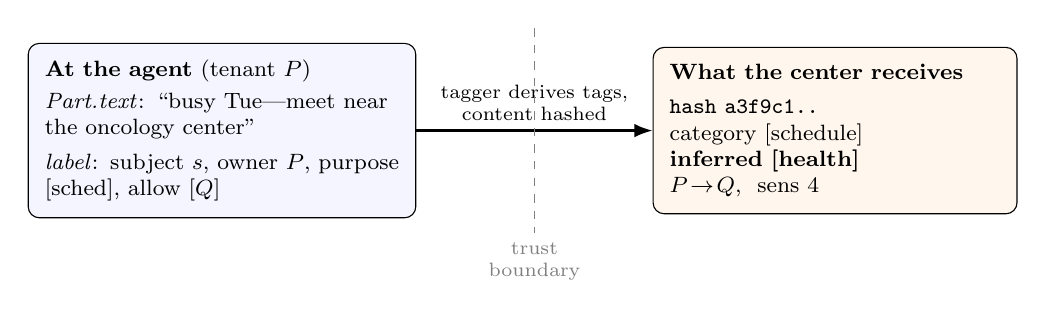
\begin{tikzpicture}[font=\footnotesize,
  raw/.style={draw,rounded corners,align=left,fill=blue!4,inner sep=6pt,text width=45mm},
  edge/.style={draw,rounded corners,align=left,fill=orange!7,inner sep=6pt,text width=42mm},
  ar/.style={-{Latex},thick}]
\node[raw] (r) {\textbf{At the agent} (tenant $P$)\\[2pt]
  \emph{Part.text}: ``busy Tue---meet near the oncology center''\\[3pt]
  \emph{label}: subject $s$, owner $P$, purpose [sched], allow [$Q$]};
\node[edge,right=30mm of r] (e) {\textbf{What the center receives}\\[3pt]
  \texttt{hash a3f9c1..}\\ category [schedule]\\ \textbf{inferred [health]}\\
  $P\!\rightarrow\!Q$, \ sens 4};
\draw[ar] (r) -- node[above,align=center,font=\scriptsize]
  {tagger derives tags,\\ content hashed} (e);
\coordinate (m) at ($(r.east)!0.5!(e.west)$);
\draw[dashed,gray] ($(m)+(0,13mm)$) -- ($(m)+(0,-13mm)$)
  node[below,gray,font=\scriptsize,align=center]{trust\\ boundary};
\end{tikzpicture}
\caption{Desensitization at the edge. The local tagger turns a benign-looking
message into governance tags (here it infers \texttt{health} from a scheduling
note) and the content is hashed; only the right-hand edge---no text---crosses the
trust boundary to the center. Recovering the message from it is infeasible
(Lemma~\ref{lem:blind}).}
\label{fig:desens}
\end{figure*}

This is the formal content of ``center-blind'': the auditor operates on a metadata
graph carrying $O(\log)$ bits per message, not a transcript. Four detectors run
over this graph:
\begin{enumerate}
\item \textbf{Cross-tenant disclosure}: sensitive data ($\geq\tau$) reaches a
principal that neither owns it nor is an allowed recipient.
\item \textbf{Purpose limitation}: data reaches an agent whose clearance purposes
are disjoint from the data's permitted purposes.
\item \textbf{Hop/TTL}: a datum (tracked by \texttt{provenance\_id}) is relayed
more than \texttt{ttl\_hops} times; robust to a forwarder re-wording content.
\item \textbf{Cross-tenant inference}: no single edge is a disclosure, but a
recipient principal accumulates converging \texttt{inferred\_categories}
fragments about one subject, letting it infer a sensitive category it was never
authorized for (Figure~\ref{fig:infer}); we ground this in the bound below.
\end{enumerate}

\begin{figure*}[t]\centering
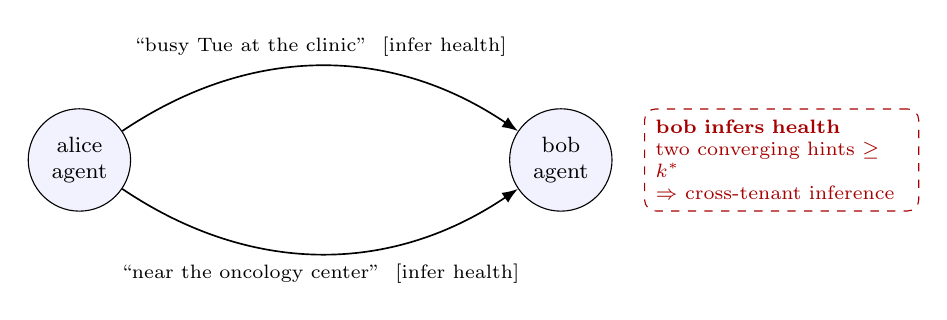
\begin{tikzpicture}[font=\footnotesize,
  ag/.style={draw,circle,align=center,fill=blue!5,inner sep=1pt,minimum size=13mm},
  ed/.style={-{Latex},semithick}]
\node[ag] (A) {alice\\ agent};
\node[ag,right=48mm of A] (B) {bob\\ agent};
\draw[ed] (A) to[bend left=34] node[above,font=\scriptsize]
  {``busy Tue at the clinic'' \ [infer health]} (B);
\draw[ed] (A) to[bend right=34] node[below,font=\scriptsize]
  {``near the oncology center'' \ [infer health]} (B);
\node[draw,dashed,rounded corners,red!65!black,align=left,right=4mm of B,
  font=\scriptsize,text width=32mm,inner sep=4pt]
  {\textbf{bob infers health}\\ two converging hints $\ge k^{*}$\\
   $\Rightarrow$ cross-tenant inference};
\end{tikzpicture}
\caption{Cross-tenant inference. Neither scheduling message leaks a sensitive
value, and bob is an allowed recipient of both; but the two hints converge on the
same subject, and their accumulated evidence crosses the detection threshold
(Prop.~\ref{prop:k})---flagged from the labels alone, no content read.}
\label{fig:infer}
\end{figure*}

\paragraph{A formal inference-gain bound.} We model what a recipient infers about
a subject's sensitive attribute $A\in\{0,1\}$ from $k$ converging fragments
$f_1,\dots,f_k$, with prior $p_0=P(A{=}1)$ and odds $O_0=p_0/(1-p_0)$.

\begin{assumption}[Conditional independence]\label{as:ci}
Given $A$, the fragments are independent, each with likelihood ratio
$\lambda_i=\tfrac{P(f_i\mid A{=}1)}{P(f_i\mid A{=}0)}\ge1$; write $\lambda$ for a
common lower bound $\lambda_i\ge\lambda>1$.
\end{assumption}

\begin{proposition}\label{prop:k}
Under Assumption~\ref{as:ci} the posterior odds are $O_k=O_0\prod_i\lambda_i$, the
posterior is $P(A\mid f_{1:k})=O_k/(1+O_k)$, and the inference gain
$g(k)=P(A\mid f_{1:k})-p_0$ is strictly increasing in $k$. With uniform $\lambda$,
the detector (fires iff $g(k)\ge\delta$) fires exactly for
$k\ge k^{*}=\big\lceil\log_\lambda(O_\delta/O_0)\big\rceil$, where
$O_\delta=(p_0+\delta)/(1-p_0-\delta)$.
\end{proposition}
\begin{proof}
By Bayes in odds form, $O_k=O_0\prod_i\lambda_i$; since each $\lambda_i>1$, $O_k$
is strictly increasing in $k$, and $x\mapsto x/(1+x)$ is strictly increasing, so
$g$ is strictly increasing. With uniform $\lambda$, $g(k)\ge\delta \iff
P(A\mid f_{1:k})\ge p_0+\delta \iff O_k\ge O_\delta \iff O_0\lambda^{k}\ge O_\delta
\iff k\ge\log_\lambda(O_\delta/O_0)$; integrality gives the ceiling.
\end{proof}
For defaults $(p_0,\lambda,\delta)=(0.1,3,0.3)$, $k^{*}=2$: one hint never fires,
two converging fragments do (posterior $0.50$, gain $0.40$), replacing the
heuristic $1-2^{-k}$ with a calibrated quantity and a closed-form bound (Figure~\ref{fig:gain});
deployments tune $(p_0,\lambda,\delta)$ and may set $\lambda_i$ from the tagger's
hint specificity (so one high-$\lambda$ fragment can suffice).
\emph{On the assumption:} real fragments are correlated, so
Assumption~\ref{as:ci} is an approximation --- positively-correlated (redundant)
hints make the true joint ratio smaller than $\prod\lambda_i$, so the model can
over-credit evidence; empirically the detector nonetheless \emph{under}-fires
relative to a real LLM recipient, because tagger coverage, not the bound, is the
binding constraint. The bound is thus a calibrated design tool, not a tight
guarantee.

\begin{figure}[t]\centering
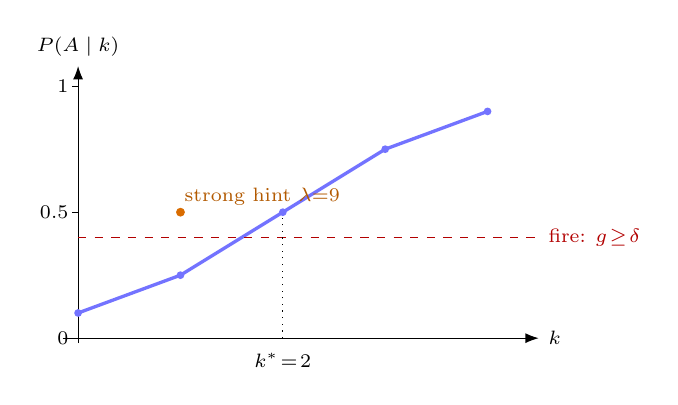
\begin{tikzpicture}[font=\footnotesize,x=13mm,y=32mm]
\draw[-{Latex}] (-0.15,0) -- (4.5,0) node[right,font=\scriptsize]{$k$};
\draw[-{Latex}] (0,-0.02) -- (0,1.08) node[above,font=\scriptsize]{$P(A\mid k)$};
\foreach \y in {0,0.5,1} \draw (-0.06,\y)--(0,\y) node[left,font=\scriptsize]{\y};
\draw[very thick,blue!55] (0,0.1)--(1,0.25)--(2,0.5)--(3,0.75)--(4,0.9);
\foreach \k/\p in {0/0.1,1/0.25,2/0.5,3/0.75,4/0.9} \fill[blue!55] (\k,\p) circle(1.4pt);
\draw[dashed,red!70!black] (0,0.4)--(4.5,0.4)
  node[right,font=\scriptsize,red!70!black]{fire: $g\!\ge\!\delta$};
\draw[dotted] (2,0)--(2,0.5); \node[below,font=\scriptsize] at (2,-0.02){$k^{*}\!=\!2$};
\fill[orange!85!black] (1,0.5) circle(1.6pt);
\node[orange!70!black,font=\scriptsize,above right=-1pt and -2pt] at (1,0.5){strong hint $\lambda{=}9$};
\end{tikzpicture}
\caption{The inference threshold. Under uniform evidence ($p_0{=}0.1,\lambda{=}3,
\delta{=}0.3$) the posterior crosses the fire line at $k^{*}{=}2$: one hint is
tolerated, two converge. A single high-specificity hint ($\lambda{=}9$, from the
tagger) already clears it.}
\label{fig:gain}
\end{figure}

\section{The A2A-MT benchmark}
No multi-tenant agent-privacy benchmark exists---AgentLeak and Sum-Leaks are
single-tenant (the vault belongs to one system; the boundary is system$\rightarrow$output).
A2A-MT supplies labeled multi-tenant A2A interactions whose boundary is
\emph{between} agents. A curated \emph{calendar-negotiation} family (two people's
scheduling agents must reveal availability without leaking \emph{why} a slot is
blocked) instantiates all four violation types; parameterized families
(group-assistant, marketplace-delegation, cross-tenant aggregation, plus
disclosure, purpose, TTL, and inference sweeps with near-miss clean controls) give 48
labeled scenarios, ground truth set by template intent. An LLM fills each Part
with realistic text matching its label (labels remain the ground truth), exported
as a shareable artifact.

\section{Evaluation}\label{sec:eval}
We ask whether the auditor detects multi-tenant leaks accurately and
without seeing content; how it fares against the tools a practitioner would
actually deploy; whether the result survives once we stop grading our own work;
and whether the compositional threat it targets is real.

\subsection{Detection and center-blindness}
Over all 48 A2A-MT scenarios, $P/R/F1 = 1.0$
(TP$=18$, FP$=0$, TN$=30$, FN$=0$) with full per-type coverage (disclosure,
purpose, TTL, inference), and no over-firing on single-hint clean controls.
 Zero raw \texttt{Part} content reaches the center
on every scenario; the only content-derived value is a one-way hash.

\subsection{Realistic content}
Re-auditing the LLM-generated export (non-templated
text) holds $P/R/F1 = 1.0$, $0$ raw leaks: the detectors key on labels, not
wording. Generating realistic content also exposed two correctness issues that
hand-written tests hid (TTL fragility to paraphrasing, fixed by
\texttt{provenance\_id}; an invariant false-positive on prose tokens coinciding
with label/schema tokens, fixed by excluding them), a benefit of scaling.

\subsection{Adaptive evasion, and closing the gap}
An adversary that knows the inference detector is
tested across evasions (Table~\ref{tab:evasion}). The design resists attacks on
\emph{wording and routing}; it is evaded only by a dishonest \emph{local} labeler
(suppressing tags or forging subject ids)---the trust assumption removed by
forced-embed attestation and canonical owner-issued subject ids. Sub-threshold
leakage evades only by leaking strictly less. We \emph{implement} this defense:
the auditor+tagger ship as a build-pinned component whose key is held only by the
unmodified binary, and the center accepts a report only from a trusted build
fingerprint. Under-tagging and forgery require modifying the labeler, so the
report is signed by an untrusted build and is \textbf{rejected}; tampering is
caught by an edges-hash mismatch; canonical owner-derived subject ids
(\texttt{canonical\_subject}) make aliasing impossible without abandoning the
attested derivation. The evasions become detected non-compliance, leaving only
key compromise (the TEE regime) as residual---the guarantee stated formally in
Prop.~\ref{prop:attest} (\S\ref{sec:threat}).

\begin{table*}[t]\centering\small
\begin{tabular}{lc}
\toprule
Evasion strategy & Result \\
\midrule
Paraphrase each fragment & resisted (tag-based, not text) \\
Split across recipient's agents & resisted (grouped by principal) \\
Partial under-tag ($\geq2$ tagged) & resisted \\
Sub-threshold (leak 1 fragment) & evades, but leaks less \\
Under-tag ($1$ of $3$) & evades $\rightarrow$ needs attestation \\
Subject-id forgery & evades $\rightarrow$ needs canonical ids \\
\bottomrule
\end{tabular}
\caption{Adaptive evasion vs.\ the inference detector.}
\label{tab:evasion}
\end{table*}

\subsection{Metadata privacy under differential privacy}
Beyond hiding content, we harden the
metadata: identity-bearing fields are pseudonymized with a per-audit shared salt
(cross-tenant comparisons hold in pseudonym space; the center learns no real
identity) and \texttt{sensitivity} is DP-noised, while categories are kept
structurally. Pseudonymization is lossless ($P/R/F1=1.0$); with DP,
$F1 = 0.99/0.97/0.96$ at $\varepsilon = 3/1/0.5$, recall falling only for
disclosure decisions whose sensitivity noises across the floor, with zero raw
content at every $\varepsilon$.

\subsection{Comparison with real baselines}
Against the two detectors a
practitioner would actually reach for (Table~\ref{tab:frontier}, 8 realistic
scenarios spanning PII disclosure, no-PII inference, and authorized sharing):
\emph{structurally}, both baselines must ingest content while ours ingests none, the disqualifier
for regulated, cross-tenant deployments, independent of
accuracy. \emph{On accuracy}, the DLP scanner is blind to no-PII inference (0\%
recall) and over-flags authorized cross-boundary sharing; a single-shot
policy-aware LLM-judge is unreliable on compositional inference across messages
(0\%, $F1=0.57$). Ours reaches full detection at zero content, the LLM tagger
lifting the honest lexical floor $0.89\to1.0$.

\begin{table*}[t]\centering\small
\begin{tabular}{lccc}
\toprule
Detector & F1 & inference rec. & content$\to$center \\
\midrule
DLP / PII scanner (sees content) & 0.67 & 0\% & 439 ch \\
LLM-judge, policy-aware (reads all) & 0.57 & 0\% & 439 ch \\
Ours --- lexical tagger (blind) & 0.89 & 50\% & \textbf{0} \\
\textbf{Ours --- LLM tagger (blind)} & \textbf{1.00} & \textbf{100\%} & \textbf{0} \\
\bottomrule
\end{tabular}
\caption{Ours vs.\ real baselines on realistic scenarios.}
\label{tab:frontier}
\end{table*}

\subsection{The local tagger}
The inference
detector accumulates \texttt{inferred\_categories}; in a real deployment these
must be \emph{produced} from content, not hand-set. A local tagger (lexical,
zero-dependency, optional LLM backend) emits only tags---content never leaves the
agent. On a labeled set with paraphrased cases, the lexical backend recovers explicit
(sensitive) \texttt{category} at $P/R/F1=1.0$ and \texttt{inferred\_categories}
at $P=1.0$, $R=0.78$; the \textbf{LLM backend (gpt-4o-mini) lifts inferred-category
recall $0.78\to1.0$} (the misses are novel paraphrases like ``the place where they
treat tumors'').
\texttt{AuditSession.observe} wires it in so a deployer supplies only text plus
policy. Tagger recall is exactly the residual surface identified above (an
adversarial sender can under-tag), which attestation closes.

\subsection{External validation on AgentLeak}
The multi-tenant
auditor reuses a federated engine we validate on the external \textbf{AgentLeak}
benchmark. Driving AgentLeak's own 600 multi-agent scenarios through an LLM to
produce real inter-agent traces and labeling leakage by AgentLeak's rule, the
auditor detects \textbf{100\% of internal-channel leaks at 0.972 precision with
zero raw vault content reaching the center} ($82.5\%$ internal-channel leak rate,
matching AgentLeak). On a labeled 33-scenario set the engine holds $P/R/F1=1.0$,
and under the full six-layer desensitizer plus DP it holds $F1\approx0.97$ at
$\varepsilon\in[0.5,3]$ with zero raw leakage, the privacy--utility result the
multi-tenant typing builds on.

\subsection{Agents in the wild}
Away from any labeled benchmark, we measure how real agents behave: 24 realistic
multi-agent workflows across 7 domains, each holding a sensitive record, where a
coordinator agent is asked to delegate to an \emph{external} specialist with no
engineered leaks, run 5$\times$ each (120 trials) for \emph{each} of four recipient
models spanning open-weight (Qwen2.5-7B/14B, Llama-3.1-8B) and frontier
(Claude~Opus~4.8). Over-sharing is prevalent across every model and, revealingly,
\emph{falls with capability but never disappears}: the open models leak the subject's
sensitive identifiers (SSN, MRN, account/card numbers, diagnoses) in \textbf{78--82\%}
of trials, the aligned frontier model in \textbf{46\%} (Table~\ref{tab:wild}). Every
cross-purpose hand-off is a purpose violation by construction, and the center-blind
auditor flagged all of them with \textbf{zero raw content reaching the center on every
model}. This is the deployment-measurement counterpart to AgentLeak on the
multi-tenant setting: left to their own judgment, current agents---weak and strong
alike---routinely over-share a subject's identifiers across organizational boundaries,
and the auditor catches it without seeing the data.

\begin{table}[t]\centering\small
\begin{tabular}{llcc}
\toprule
Recipient model & tier & disclosure & raw$\to$center \\
\midrule
Qwen2.5-7B   & small (open) & 82\% (99/120) & \textbf{0} \\
Llama-3.1-8B & small (open) & 81\% (97/120) & \textbf{0} \\
Qwen2.5-14B  & mid (open)   & 78\% (94/120) & \textbf{0} \\
\textbf{Claude Opus~4.8} & frontier & \textbf{46\% (55/120)} & \textbf{0} \\
\bottomrule
\end{tabular}
\caption{Cross-boundary over-sharing by recipient model (24 workflows $\times$ 5 runs
$=120$ trials each, same set). Over-sharing falls with capability/alignment but stays
high; the auditor catches all at zero content egress.}
\label{tab:wild}
\end{table}

\subsection{An author-independent benchmark}
Our 48-scenario benchmark scores
1.0, but we wrote both the detectors and the scenarios. To de-bias it, an LLM
(\emph{not} the detector author) generates diverse scenarios with its own intended
labels and we score our auditor against them. Across held-out runs ($\approx$20
scenarios each), \textbf{precision is 1.0 (the architecture never over-fires) but
recall is only $\approx$0.31 (lexical) / 0.38 (LLM tagger)}, far below the
self-authored 1.0. The misses are dominated by tagger/taxonomy coverage: we
broaden the sensitive set from health/finance/legal to ten configurable classes
(+location, employment, education, behavioral, credentials, biometric,
demographic), which raises recall, but open-world sensitive content remains the
bottleneck; the author also states inferences explicitly and labels some
borderline cases as leaks. Recall here is bounded by the tagger, an orthogonal
and improvable component, not the auditor: every violation the
architecture reports is real. The self-authored 1.0 measures the detectors given
correct labels; the held-out setting measures the end-to-end pipeline on
open-world content.

\subsection{Is the inference threat real?}
Our detector fires at $k^{*}=2$ hints, but is that where real inferability begins? We
have an independent LLM play the recipient and infer the subject's withheld attribute
from the $K$ benign fragments it received ($K=1,2,3$), scaled to \textbf{16 sensitive
attributes} across health, finance, employment, legal, and behavioral domains
($5$ trials each). \emph{The threat is real, and for a frontier recipient it begins
below our threshold:} Claude Opus~4.8 infers the withheld attribute from two benign
fragments in \textbf{100\% (16/16)} of attributes and from a \emph{single} fragment in
\textbf{81\% (13/16)}. Weaker recipients need more evidence: on the same 16-attribute
set, open-weight recipients infer at $K{=}2$ in 56--69\% (Qwen2.5-7B, Llama-3.1-8B)
and 81\% (Qwen2.5-14B) of attributes, versus 100\% for the frontier model---inference
at the detection threshold rises with capability, so the compositional threat grows as
agents improve. \emph{This makes our detector
a conservative, no-false-alarm lower bound:} it stays silent at $K=1$, yet a strong
recipient already infers there; every disagreement is an under-fire, and we never fire
where the recipient cannot infer. Hence detection must flag the metadata pattern, not
try to out-infer the adversary. The
threshold $k^{*}=2$ with uniform evidence is conservative: real inference sometimes needs one high-specificity hint, which
the Bayesian model of \S\ref{sec:auditor} accommodates via a per-fragment
$\lambda$; wiring
$\lambda$ to hint specificity catches single strong hints without over-firing.

\section{Discussion}
Center-blind detection works because the risks it targets are visible in the
metadata graph (principals, categories, inferred-category tags, provenance), all
of which the local side can emit without revealing content. The same observation
explains why the system is at once a research result and a product: set every
owning principal equal and the multi-tenant model collapses to the in-container
case, where the identical detectors flag a sensitive datum crossing to an agent or
tool it should not reach, still without shipping content anywhere.

\begin{figure}[t]\centering
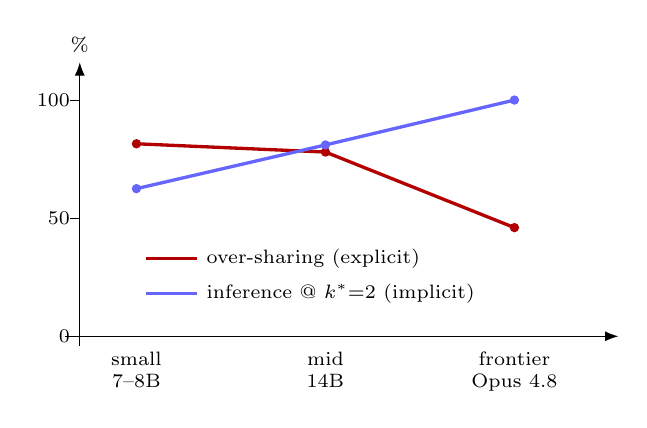
\begin{tikzpicture}[font=\footnotesize,x=24mm,y=0.30mm]
\draw[-{Latex}] (0.62,0) -- (3.55,0);
\draw[-{Latex}] (0.7,-4) -- (0.7,116) node[above,font=\scriptsize]{\%};
\foreach \y in {0,50,100} \draw (0.65,\y)--(0.7,\y) node[left,font=\scriptsize]{\y};
\foreach \x/\l in {1/{small\\7--8B},2/{mid\\14B},3/{frontier\\Opus 4.8}}
  \node[align=center,font=\scriptsize,below=2pt] at (\x,0) {\l};
\draw[very thick,red!70!black] (1,81.5)--(2,78)--(3,46);
\foreach \x/\y in {1/81.5,2/78,3/46} \fill[red!70!black] (\x,\y) circle(1.7pt);
\draw[very thick,blue!60] (1,62.5)--(2,81)--(3,100);
\foreach \x/\y in {1/62.5,2/81,3/100} \fill[blue!60] (\x,\y) circle(1.7pt);
\draw[very thick,red!70!black] (1.05,33)--(1.32,33);
\node[right,font=\scriptsize] at (1.32,33){over-sharing (explicit)};
\draw[very thick,blue!60] (1.05,18)--(1.32,18);
\node[right,font=\scriptsize] at (1.32,18){inference @ $k^{*}{=}2$ (implicit)};
\end{tikzpicture}
\caption{Two opposing trends across recipient capability (tier means; per-model values
in Table~\ref{tab:wild} and \S\ref{sec:eval}). As recipients get stronger,
\emph{explicit} over-sharing falls while \emph{implicit} inference rises---neither end
is safe to trust, and the center-blind auditor catches both at zero content egress.}
\label{fig:trends}
\end{figure}

Our multi-model study exposes two opposing trends that together make the case for
metadata-level detection (Figure~\ref{fig:trends}). As recipient capability rises,
\emph{explicit} over-sharing falls---weaker models paste a subject's identifiers into a
hand-off outright ($\approx$80\%), the aligned frontier model far less often
(46\%)---while \emph{implicit} inference rises: the frontier recipient reconstructs a
withheld attribute from two benign fragments where a small model cannot. A defender who
trusted the model to behave would be wrong at both ends. The auditor does not: it flags
the metadata pattern---an explicit sensitive tag crossing a boundary, or converging
inferred-category fragments---and catches both, with zero content egress across the
whole capability range.

The honest limits lie in coverage and in trust. Recall is bounded not by the
auditor but by the tagger that feeds it: on author-independent scenarios precision
stays perfect while recall trails, because open-world sensitive content outruns
any fixed taxonomy. The inference bound assumes conditionally independent
fragments, which real, correlated hints only approximate. And two adversaries
remain open: a peer that both paraphrases \emph{and} keeps every recipient below
the convergence threshold, and a colluding sender--recipient pair that suppresses
a shared datum---the residual that only a hardware root of trust (the TEE backend
our attestation admits) fully closes.

\section{Related work}

\noindent\textbf{Privacy leakage in LLM-agent systems.} AgentLeak~\cite{agentleak}
and Sum-Leaks~\cite{sumleaks} measure and mitigate \emph{single-tenant}
compositional leakage; privacy-theory work for agents~\cite{dpagents,itlimits}
analyzes when local privacy fails to compose. LLMs also memorize and regurgitate
training data~\cite{carlini21,carlini23}. We lift the setting to \emph{multi-tenant}
and supply a deployable, center-blind detector rather than a measurement or a
theory.

\noindent\textbf{Agent communication protocols.} A2A~\cite{a2a}, MCP~\cite{mcp},
and related standards define agent interoperability but no data governance;
comparative security analyses~\cite{protosec,protoexploit} flag exactly this gap,
which we fill inside A2A's extension mechanism.

\noindent\textbf{Information-flow control and taint tracking.} Our detectors are a
lightweight, semantic information-flow analysis: the lattice model~\cite{denning76}
and language-based IFC~\cite{sabelfeld03} formalize where data may flow, and
dynamic taint tracking~\cite{taintdroid} enforces it at runtime. We adapt these to
opaque LLM agents over metadata (not program variables), adding purpose and
cross-tenant semantics and \emph{compositional inference}, which classical IFC
does not model. Purpose- and recipient-limitation follow the norm of contextual
integrity~\cite{ci}.

\noindent\textbf{Data-loss prevention.} DLP / PII scanners (e.g.\
Presidio~\cite{presidio}) match sensitive patterns in content; they see raw data,
have no policy/purpose semantics, and are blind to no-PII inference (\S\ref{sec:eval}). We are
center-blind and compositional.

\noindent\textbf{Anonymization and differential privacy.} $k$-anonymity~\cite{ksweeney}
and $\ell$-diversity~\cite{ldiv} motivate our structural domain generalization;
differential privacy~\cite{dwork06,dworkroth} and local DP~\cite{rappor} underlie
our metadata hardening (\S\ref{sec:eval}). Unlike these, our object is \emph{detection} of a
composed leak, not release of a sanitized dataset.

\noindent\textbf{Federated and secure computation.} The federated split follows
federated learning's keep-data-local principle~\cite{fedavg}; stronger guarantees
are available via secure computation~\cite{yao} and trusted execution, which our
attestation layer (\S\ref{sec:eval}) plugs into. We target a deployable software baseline with a
TEE upgrade path.

\noindent\textbf{Observability.} LangSmith and Langfuse~\cite{langfuse} trace
agent runs but must ingest raw prompts and outputs, the disqualifier for
regulated, cross-tenant deployments and the one property our design structurally
avoids.

\section*{Ethical Considerations}
This work involves no human subjects and required no IRB review. Every scenario is
synthetic: the A2A-MT benchmark and the in-the-wild study use LLM-generated content
populated with fictional identifiers (invented names and format-valid but
non-real SSNs, MRNs, and account numbers), and the external validation runs on the
already-public AgentLeak benchmark. No real personal data is collected, stored, or
transmitted. The artifact is defensive by construction and center-blind in
operation: it detects privacy violations from desensitized metadata and, by design,
no raw content reaches the central component even in deployment. We considered
dual-use: our threat model and inference detector describe how compositional
leakage arises, but that same analysis is what a defender needs, and we disclose no
attack beyond what AgentLeak and Sum-Leaks already document. No component met the
threshold for an external ethics panel; we are glad to clarify any concern with the
program committee.

\section*{Open Science}
The full system---the \ext{} extension, the center-blind auditor and its four
detectors, the local tagger, the attestation layer---and the A2A-MT benchmark
generator are implemented and will be released under an open-source license upon
publication, together with scripts that reproduce every quantitative result in
Section~\ref{sec:eval}. For double-blind review we provide an anonymized snapshot at
\url{https://anonymous.4open.science/r/a2a-mt-audit} with identifying information
removed. The benchmark is exported as a versioned, shareable artifact so results are
reproducible independently of our implementation, and we intend to submit it for
artifact evaluation.

\section*{Use of AI-Based Tools}
AI-based tools were used both as part of our research methodology and in preparing
this manuscript. \emph{Methodology (described in the paper):} the local tagger
optionally uses an LLM backend (gpt-4o-mini) to derive privacy tags
(\S\ref{sec:eval}); the A2A-MT benchmark and the author-independent held-out set are
populated and authored by LLMs; and the threat-validation and in-the-wild experiments
use LLMs as the inferring recipient / coordinator (open-weight Qwen2.5-7B/14B and
Llama-3.1-8B, and frontier Claude Opus~4.8). \emph{Writing:}
the authors used generative AI-based tools to revise text, improve flow, and assist
with pre-submission review. We have manually verified and take full responsibility
for the accuracy, originality, and integrity of all content---including every
citation---and of the output of all AI-based tools.

\bibliographystyle{IEEEtran}
\bibliography{references}

\end{document}
